\section{WebRTC}

WebRTC (Web Real-Time Communication) is a free, open-source project providing web browsers and 
mobile applications with real-time communication via simple Application Programming Interfaces (APIs). 
It allows audio and video communication to work inside web pages by allowing direct peer-to-peer 
communication, eliminating the need to install plugins or download native apps.
It supports video, voice, and generic data to be sent between peers, allowing developers 
to build powerful voice- and video-communication solutions.~\cite{wikiWebRTC}

There are 3 primary components of the WebRTC API and each plays a unique role in WebRTC specification:

\subsubsection{MediaStream (GetUserMedia)}

The MediaStream API provides a way to access device cameras and microphones using JavaScript. 
It controls where multimedia stream data is consumed, and provides some control over the devices 
that produce the media. It also exposes information about devices able to capture and render media.

\subsubsection{RTCPeerConnection}

The Peer Connection is the core of the WebRTC standard. It provides a way for participants to 
create direct connections with their peers without the need for an intermediary 
server (beyond signalling). Each participant takes the media acquired from the media 
stream API and plugs it into the peer connection to create an audio or video feed.  
The PeerConnection API has a lot going on behind the scenes. It handles SDP negotiation, 
codec implementations, NAT Traversal, packet loss, bandwidth management, and media transfer.

\subsection{RTCDataChannel}

The RTCDataChannel API was setup to allow bi-directional data transfer of any 
type of data -- media or otherwise -- directly between peers. It was designed to mimic the 
WebSocket API, but rather than relying on a TCP connection which although reliable is high 
in latency and prone to bottlenecks, data channels use UDP-based streams with the configurability 
of the Stream Control Transmission Protocol (SCTP) protocol. This design allows the best 
of both worlds: reliable delivery like in TCP but with reduced congestion on the network like in UDP.

\subsection{Establishing the connection}

Before a peer-to-peer video call can begin, a connection between the two clients 
needs to be established. This is accomplished through signalling. Signalling falls 
outside of the realm of the WebRTC specification but is the vital first step in establishing 
an audio/video connection.

\subsection{Signalling}

Signalling allows two endpoints (senders, receivers, or both) to exchange metadata to 
coordinate communication in order to set up a call. This call-and-response message flow 
contains critical details about the streaming that will take place, that is, the number 
and types of streams, how the media will be encoded, etc. 

This is needed for two reasons: because the communicating peers do not know each other’s 
capabilities, and the peers do not know each other’s network addresses.

\subsection{NAT Traversal - ICE, TURN and STUN}

Once the initial signalling for a streaming connection has taken place, the two endpoints need 
to begin the process of NAT (Network Address Translation) traversal.
This assigns a public address to a computer inside a private network for setting up a real-time connection. 
In a WebRTC-enabled communication, unless the two endpoints are on the same local network, 
there will be one or more intermediary network devices (routers/gateways) between the two. 
There are three key specifications that are used in WebRTC to overcome these hurdles:

\begin{itemize}
    \item \textbf{Interactive Connectivity Establishment (ICE)} - ICE is used to find all the ways 
    for two computers to “talk to each other”. It has two main roles, gathering candidates 
    and checking connectivity. It guarantees that if there is a path for two clients to communicate, 
    it will find it and ensure it is the most efficient. It makes use of two protocols - STUN and TURN.
    \item  \textbf{Session Traversal Utilities for NAT (STUN)}  – It is a lightweight and simple 
    method for NAT Traversal. STUN allows WebRTC clients to find out their own public IP address 
    by making a request to a STUN server. 
    \item  \textbf{Traversal Using Relays around NAT (TURN) }  - The TURN server assists in the NAT 
    traversal by helping the endpoints learn about the routers on their local networks, 
    as well as blindly relaying data for one of the endpoints where a direct connection is 
    not possible due to firewall restrictions.
\end{itemize}

\begin{figure}
\begin{center}
    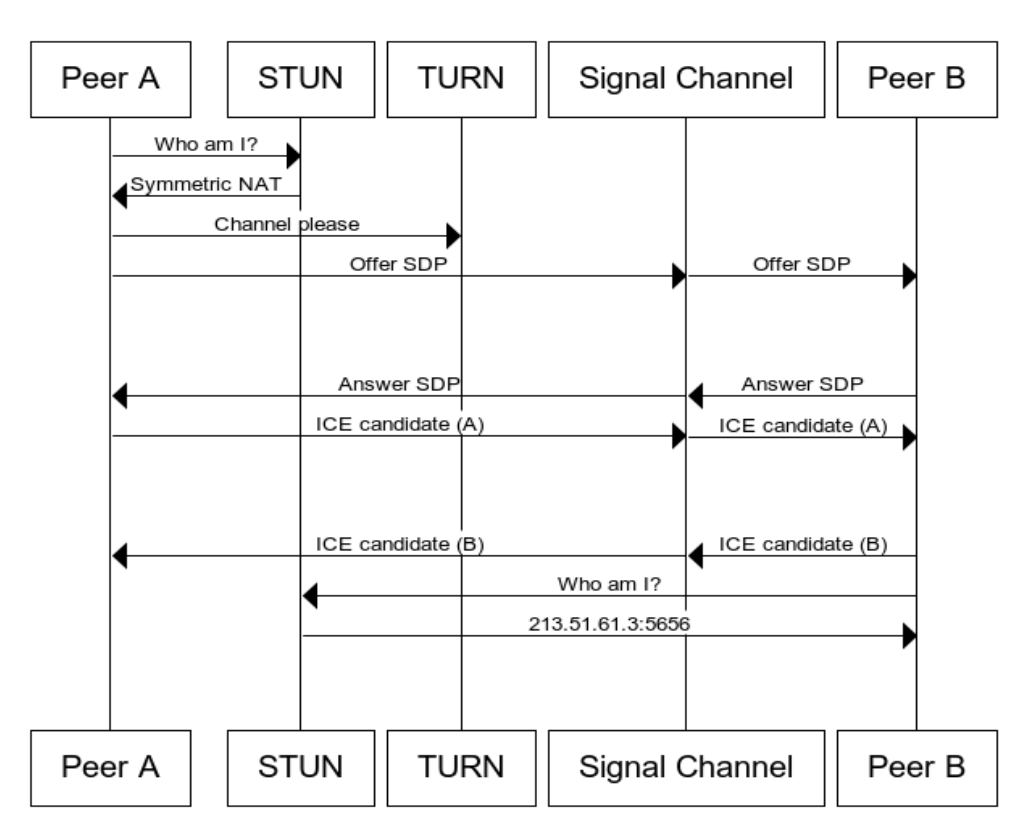
\includegraphics[width=10cm]{webRTC.png}
\end{center}
\caption{Call Service: webRTC Signalling Plane}
\label{fig:webrtc}
\end{figure}

\subsection{Codecs}

Before sending the media over a peer connection, it has to be compressed. 
Raw audio and video is simply too large to send efficiently on the current Internet infrastructure.
Likewise, after receiving media over a peer connection, it has to be decompressed. 
For this, use a media codec.

WebRTC has mandated three audio codecs and two video codecs:

\begin{enumerate}
    \item Audio - PCMU (G.711$\mu$) running at 8,000Hz with a single channel (mono).
    \item Audio - PCMA (G.711a) running at 8,000Hz with a single channel (mono).
    \item Audio - Opus running at 48,000Hz with two channels (stereo).
    \item Video - VP8.
    \item Video - H.264/AVC using Constrained Baseline Profile Level 1.2.
\end{enumerate} 

The technology is available on all modern browsers as well as on native clients for
all major platforms. The technologies behind WebRTC are implemented as an open web 
standard and available as regular JavaScript APIs in all major browsers. For native clients, 
like Android and iOS applications, a library is available that provides the same 
functionality.~\cite{UltimateGuideWebRTC}

